\documentclass[xcolor=dvipsnames]{beamer}

% Packages
\usepackage{bm}


%% Theme related.
\usetheme{default}
\setbeamertemplate{navigation symbols}{}
\setbeamertemplate{frametitle}[default][center]
\setbeamertemplate{itemize items}[circle]

\definecolor{Red}{rgb}{.9,.05,.05}
\setbeamercolor{alerted text}{fg=Red}
\usefonttheme[onlymath]{serif}


%% Math
\newcommand{\Reals}{\mathbb{R}}
\newcommand{\wh}[1]{\widehat{#1}}
\newcommand{\wt}[1]{\widetilde{#1}}
\DeclareMathOperator*{\argmin}{argmin}

%% Font
\newcommand{\red}[1]{\textcolor{red}{#1}}
\newcommand{\blue}[1]{\textcolor{blue}{#1}}

\title{Laplacian Smoothing on Neighborhood Graphs}

\author{Alden Green}
\institute{Department of Statistics and Data Science \\
		   Carnegie Mellon Unviersity}
\date{}

\begin{document}
	
\begin{frame}
\titlepage
\end{frame}

\begin{frame}{Basic problem setup}
\alert{Nonparametric regression, random design}: We observe $(X_1,Y_1),\ldots,(X_n,Y_n)$, where $X_1,\ldots,X_n$ are sampled independently from density $p$, and
\begin{equation*}
Y_i = f_0(X_i) + \varepsilon_i, \quad \varepsilon_i \sim N(0,1).
\end{equation*}
Goal is to learn the unknown regression function $f_0$, which is assumed to be \alert{Sobolev} smooth, i.e.
\begin{equation*}
\|f_0\|_{H^1}^2 := \int \|\nabla f_0(x)\|^2 \,dx \quad \text{is small.}
\end{equation*}
Either \alert{estimate} $f_0$ with some $\hat{f}$, or \alert{test} whether $f_0 = 0$.
\end{frame}

\begin{frame}{Laplacian smoothing}
Laplacian smoothing solves a discrete, penalized least squares problem on a graph.
\begin{enumerate}
	\item  Form a \alert{neighborhood graph} $G$ over $X_1,\ldots,X_n$, with weighted edges $W_{ij} = K(\|X_i - X_j\|/r)$. The \alert{graph Laplacian} $L$ is defined by
	\begin{equation*}
	(Lf)_i = \sum_{i = 1}^{n} \bigl(f(X_i) - f(X_j)\bigr) W_{ij}.
	\end{equation*}
	\item The \alert{Laplacian smoothing} estimator is
	\begin{equation*}
	\wh{f} = \argmin_{f \in \Reals^n} \|Y - f\|_n^2 + \frac{\lambda}{2} f^{\top} L f, \end{equation*}
	%with corresponding test statistic $\wh{T} = \|\wh{f}\|_n^2$.
\end{enumerate}
\begin{figure}
	\centering
	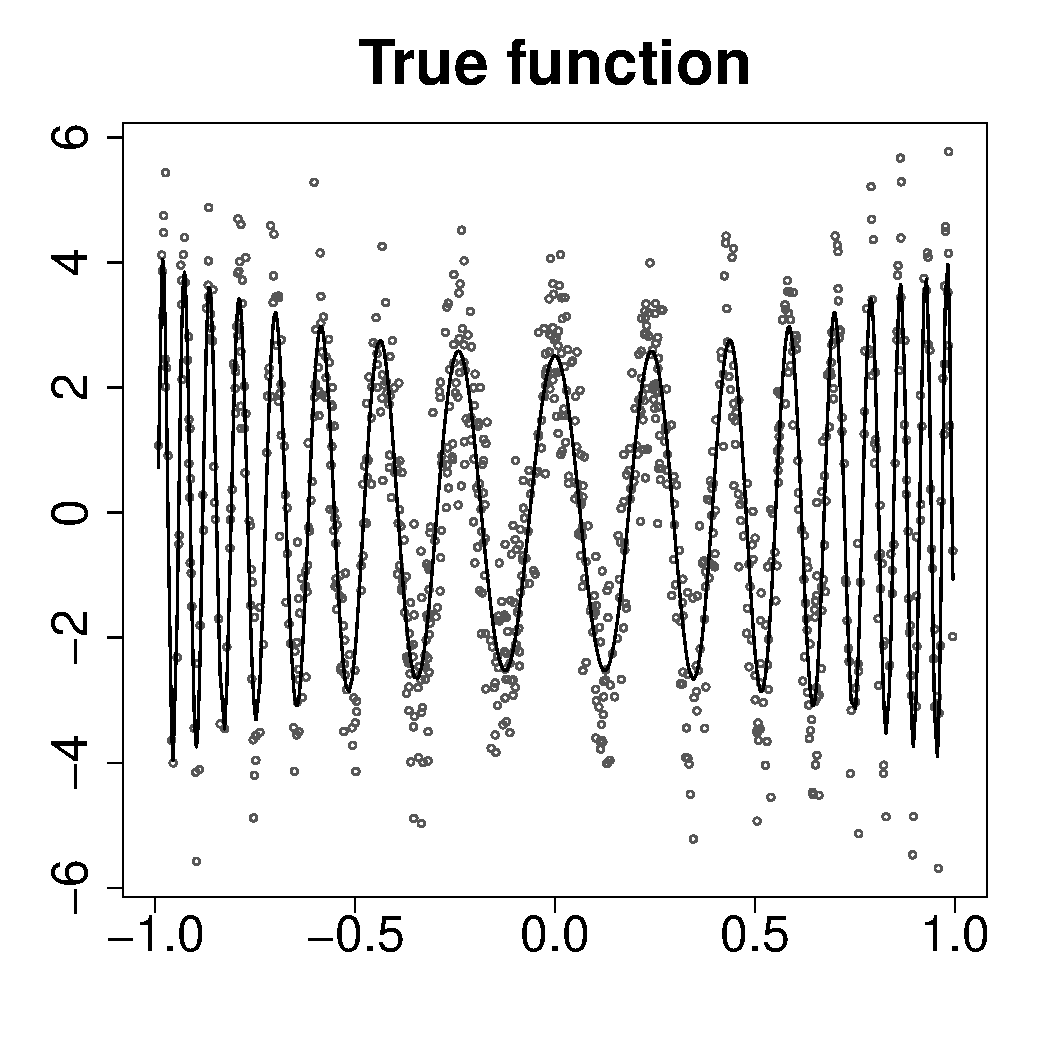
\includegraphics[width=.25\textwidth]{figures/wiggly_cosine/regression_function_1.pdf}
	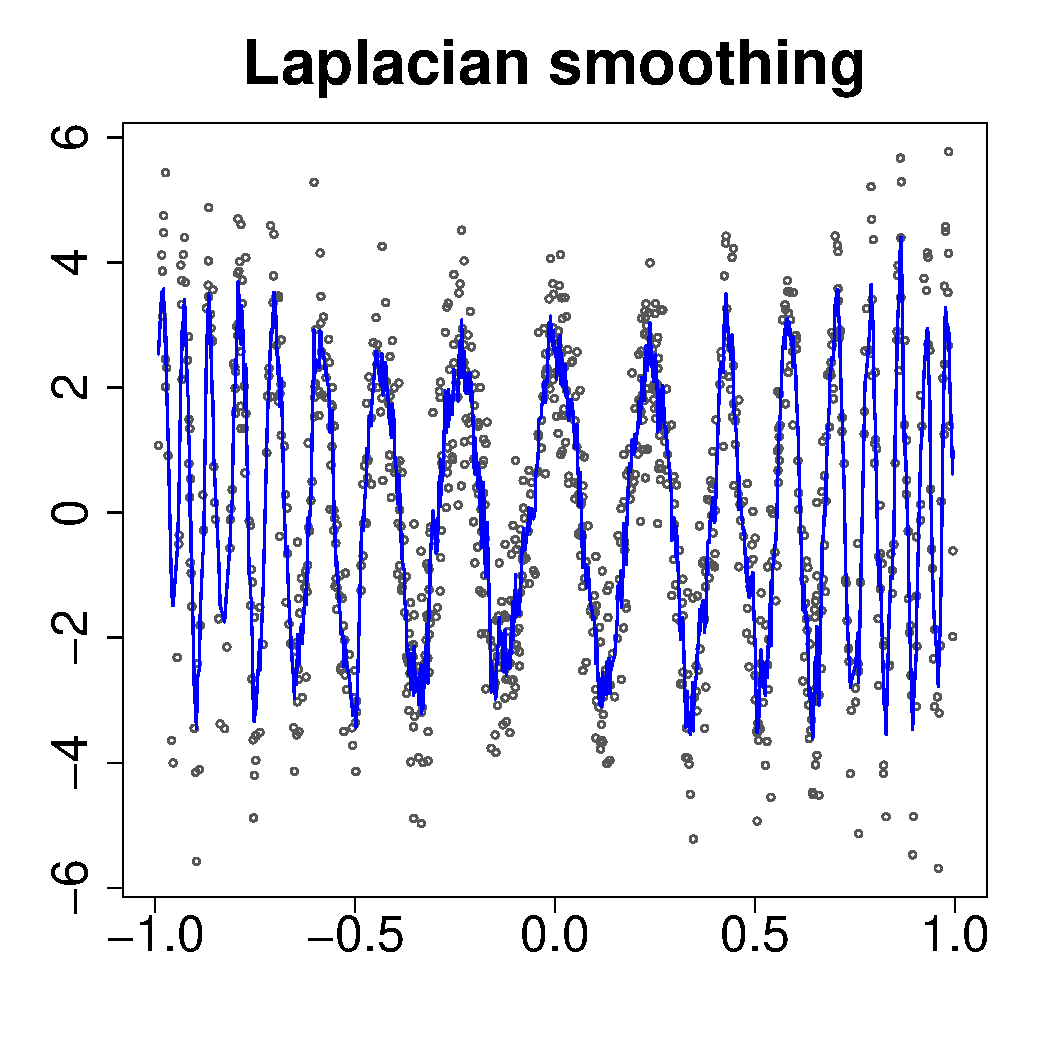
\includegraphics[width=.25\textwidth]{figures/wiggly_cosine/laplacian_smoothing_estimate_1.pdf} 
\end{figure}
\end{frame}

\begin{frame}{Motivation}
Why Laplacian smoothing?
\begin{itemize}
	\item \emph{Computational ease.} Sparse graph, fast solvers.
	\item \emph{Generality.} Makes sense whenever one can form a graph $G$. 
	\item \emph{Weak supervision.} Naturally extends to semi- and unsupervised problems.
\end{itemize}
Intuition: when $n$ large, $r$ small and $f$ smooth, \textcolor{blue}{(Bousquet et al.)} show
\begin{equation*}
f^T L f = \frac{1}{2}\sum_{i,j = 1}^{n} \bigl(f(X_i) - f(X_j)\bigr)^2 W_{i,j} \approx n^2 r^{d + 2} \int \|\nabla f\|_2^2 p^2(x) \,dx.
\end{equation*}
So $\wh{f}$ seems like a noisy approximation of a very classical estimator $\wt{f}$: aka \alert{smoothing spline} ($d = 1$), or \alert{thin-plate spline} ($d \geq 2$), defined as
\begin{equation*}
\widetilde{f} = \argmin_{f \in H^1} \|Y - f\|_n^2 + \lambda \int \|\nabla f(x)\|_2^2  \,dx.
\end{equation*}
Similarly $\wh{T}$ approximates $\wt{T} = \|\wt{f}\|_n^2$. 
\end{frame}

\begin{frame}{Main Question}
In $1d$, smoothing splines achieve the minimax optimal rate \blue{$n^{-2/3}$} (estimation) or \blue{$n^{-4/5}$} (testing) over Sobolev functions.
\begin{block}{{\bf Question}}
	Does Laplacian smoothing enjoy the same optimality properties as smoothing/thin plate splines?
\end{block}

\begin{block}{{\bf Answer}}
	They actually do better! When properly tuned:
	\begin{itemize}
		\item Laplacian smoothing has error of \blue{$n^{-2/3}$} (estimation) and \blue{$n^{-4/5}$} (testing) when $d = 1$, matching smoothing splines.
		\item Laplacian smoothing also achieves optimal error \blue{$n^{-2/(2 + d)}$} (estimation) and \blue{$n^{-4/(4 + d)}$} (testing) when $d = 2,3,4$ (up to $\log n$ factor when $d = 4$).
		\item On the other hand $\wt{f}$ is \alert{not even well-defined} when $d > 1$. Well known in spline/semi-supervised learning communities.
	\end{itemize}
\end{block}
\end{frame}

\begin{frame}{Summary of Main Results}

{\large Estimation rates, assuming $f_0 \in H^1(M)$}
\begin{table}
	\begin{center}
		\begin{tabular}{p{.25\textwidth} | p{.25\textwidth} p{.25\textwidth} }
			Dimension & Laplacian smoothing & Smoothing/Thin-plate splines \\
			\hline
			$d = 1$ & \blue{\bm{${n^{-2/3}}$}} & \blue{${n^{-2/3}}$} \\
			$d = 2,3$ & \blue{\bm{${n^{-2/(2 + d)}}$}} & \red{NA}/\red{$1$} \\
			$d = 4$ & $\bm{\blue{{n^{-1/3}}} (\log n)^{1/3}}$ & \red{NA}/\red{$1$} \\
			$d \geq 5$  & $\bm{(\log n/n)^{4/(3d)}}$ & \red{NA}/\red{$1$} \\
		\end{tabular}
	\end{center}
\end{table}

{\large Testing rates, assuming $f_0 \in H^1(M)$ ($d < 4$) or $f_0 \in L^4(M)$ ($d \geq 4$)}
\begin{table}
	\begin{center}
		\begin{tabular}{p{.25\textwidth} | p{.25\textwidth} p{.25\textwidth} }
			Dimension & Laplacian smoothing & Smoothing/Thin-plate splines \\
			\hline
			$d = 1$ & \blue{\bm{${n^{-4/5}}$}} & \blue{${n^{-4/5}}$} \\
			$d = 2,3$ & \blue{\bm{${n^{-4/(4 + d)}}$}} & \red{NA}/\red{$n^{-1/2}$} \\
			$d \geq 4$ & $\blue{\bm{{n^{-1/2}}}}$ & \red{NA}/\blue{$n^{-1/2}$} \\
		\end{tabular}
	\end{center}
\end{table}
\end{frame}

\begin{frame}{Explanation: Failure of Thin-plate Splines}
Well-posedness of smoothing splines (when $d = 1$) vs. ill-posedness of thin-plate splines ($d \geq 2$) explained by \alert{Sobolev Embedding Theorem}.
\begin{itemize}
	\item In $1d$, every function in $H^1$ is continuous. 
	\item When $d \geq 2$, this is no longer the case.
\end{itemize}
As a result the criterion underlying $\wt{f}$ is \alert{not continuous} with respect to $H^1$ norm. \blue{(Green and Silverman)} construct sequences of ``bump functions'' $f_1,f_2,\ldots$ such that
\begin{equation*}
f_k(X_i) = Y_i \quad \text{for all $i = 1,\ldots,n$, but} \quad \|f_k\|_{H^1} \to 0.
\end{equation*}
\alert{Bottom line}: The continuum thin-plate spline problem assigns (much) higher loss + penalty to the regression function $f_0$ than to bump functions $f_k$.
\end{frame}

\begin{frame}{Explanation: Success of Laplacian Smoothing}
\alert{Discretization} is a blessing!  
\begin{itemize}
	\item Previous construction of ``bump functions'' $f_1,f_2,\ldots$ will satisfy
	\begin{equation*}
	f_k^{\top} L f_k = \sum_{i,j = 1}^{n} (Y_i - Y_j)^2 K(\|X_i - X_j\|/r) \asymp n^2r^{d}.
	\end{equation*}
	\item If $f_0$ is Sobolev smooth, then $f_0^{\top} L f_0 \lesssim n^2r^{d + 2}$.
	\item Thus for $\lambda \gg (nr^{d + 2})^{-1} r^{-2}$, we have
	\begin{equation*}
	\|Y - f_k\|_n^2 + \lambda f_k^{\top} L f_k \gg \|Y - f_0\|_n^2 + \lambda f_0^{\top} L f_0.
	\end{equation*}
\end{itemize}
\alert{Bottom line}: the discrete problem assigns (much) higher loss + penalty to bump functions $f_k$ than to regression function $f_0$.
\end{frame}


\begin{frame}{What about $d > 4$?}
\alert{Estimation}: the class $H^1(G;M) = \{f: f^{\top}Lf \leq M\}$ is too large to show $\wh{f}$ is optimal. Similar phenomena in ERM over H\"{o}lder classes when $d > 2$ \blue{(Birge and Massart)}, and fixed (grid) graphs \blue{(Sadhanala et al.)}. Empirically, we see that for $f_0$ simple $\cos$ function,
\begin{figure}[tb]
	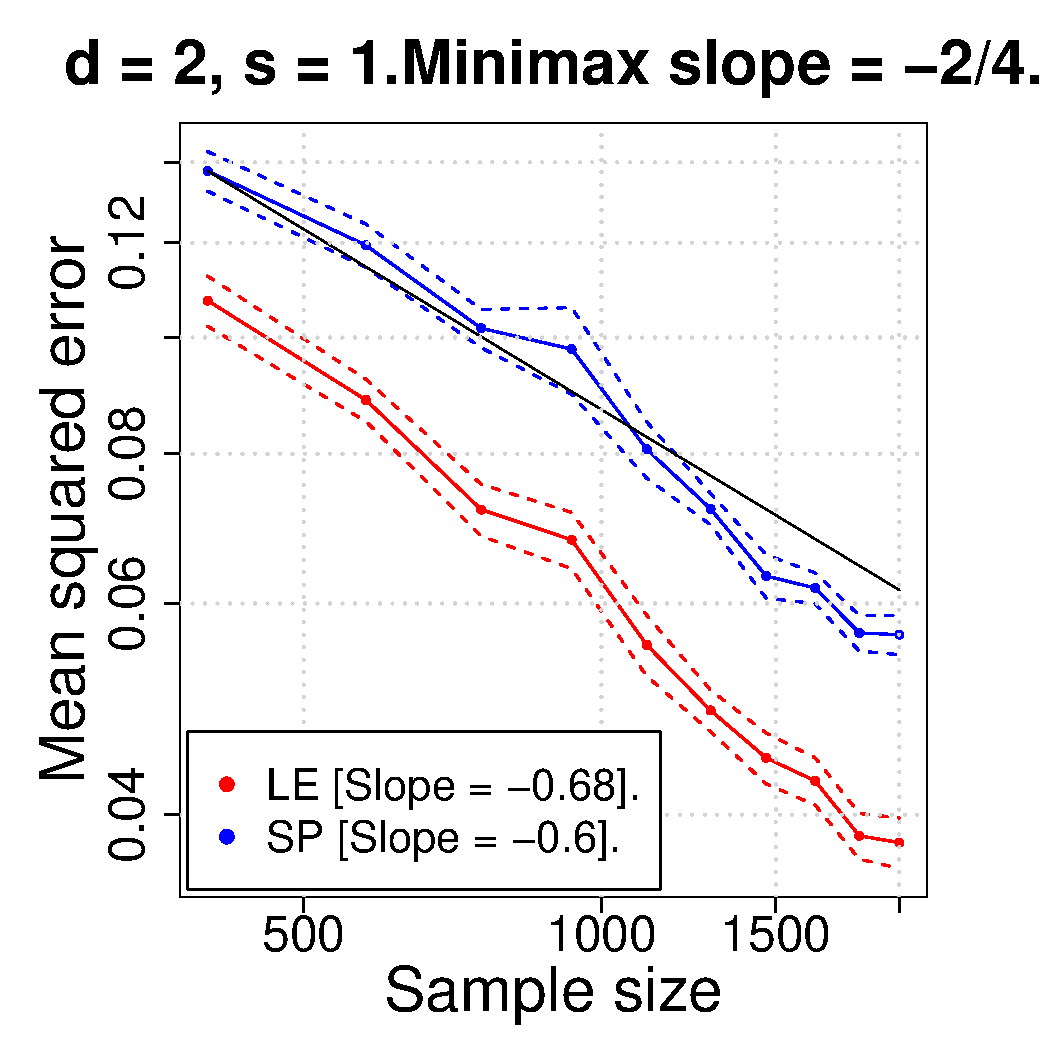
\includegraphics[width=.24\textwidth]{figures/cosine/mse_by_sample_size_2d.pdf}
	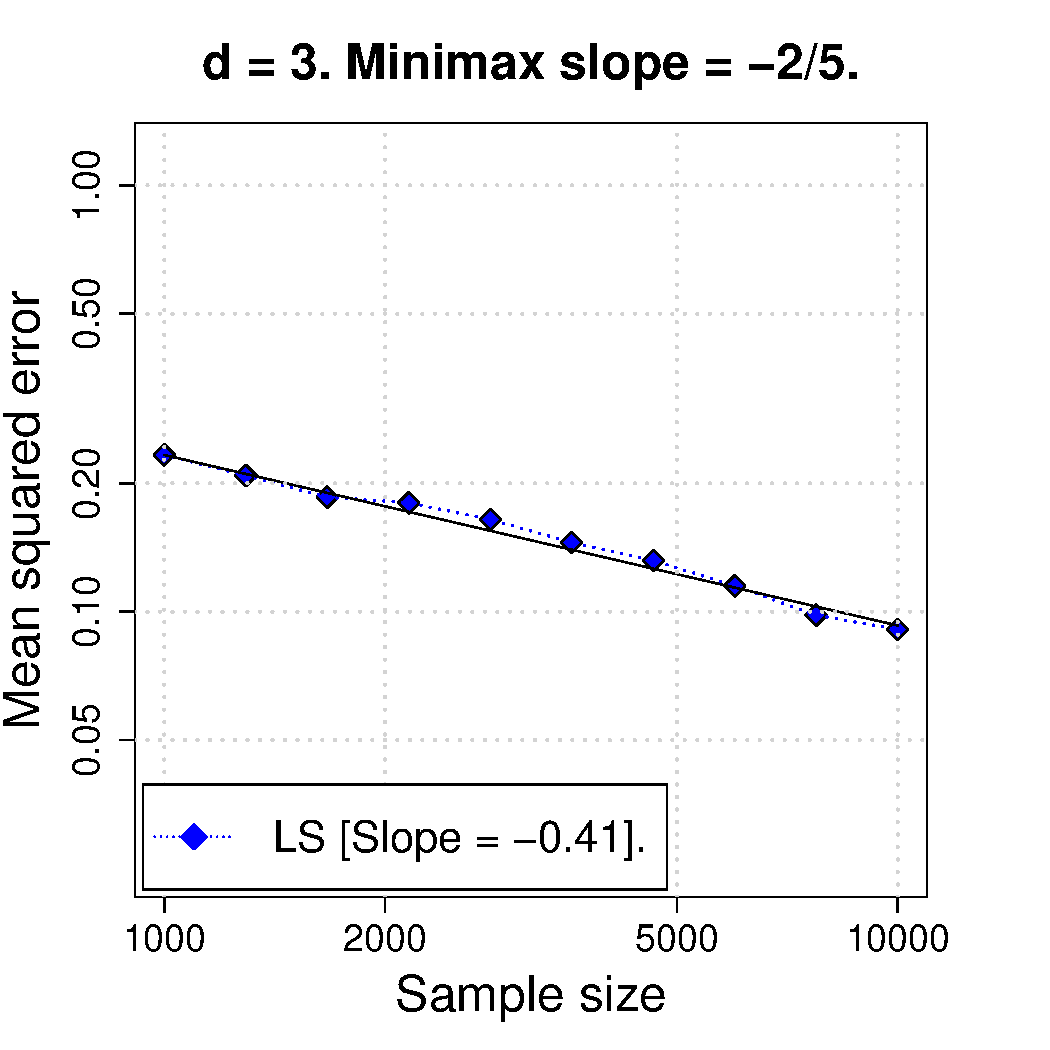
\includegraphics[width=.24\textwidth]{figures/cosine/mse_by_sample_size_3d.pdf} 
	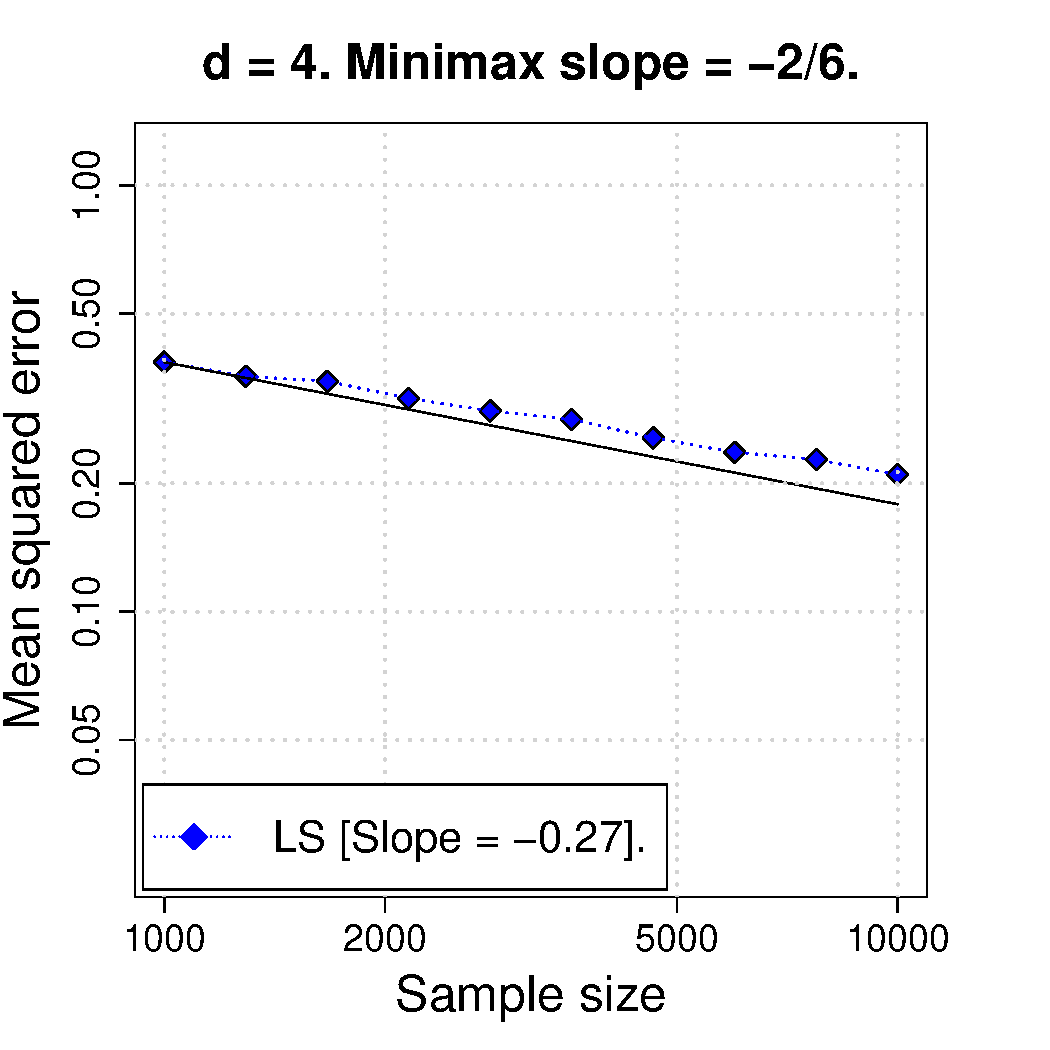
\includegraphics[width=.24\textwidth]{figures/cosine/mse_by_sample_size_4d.pdf}
	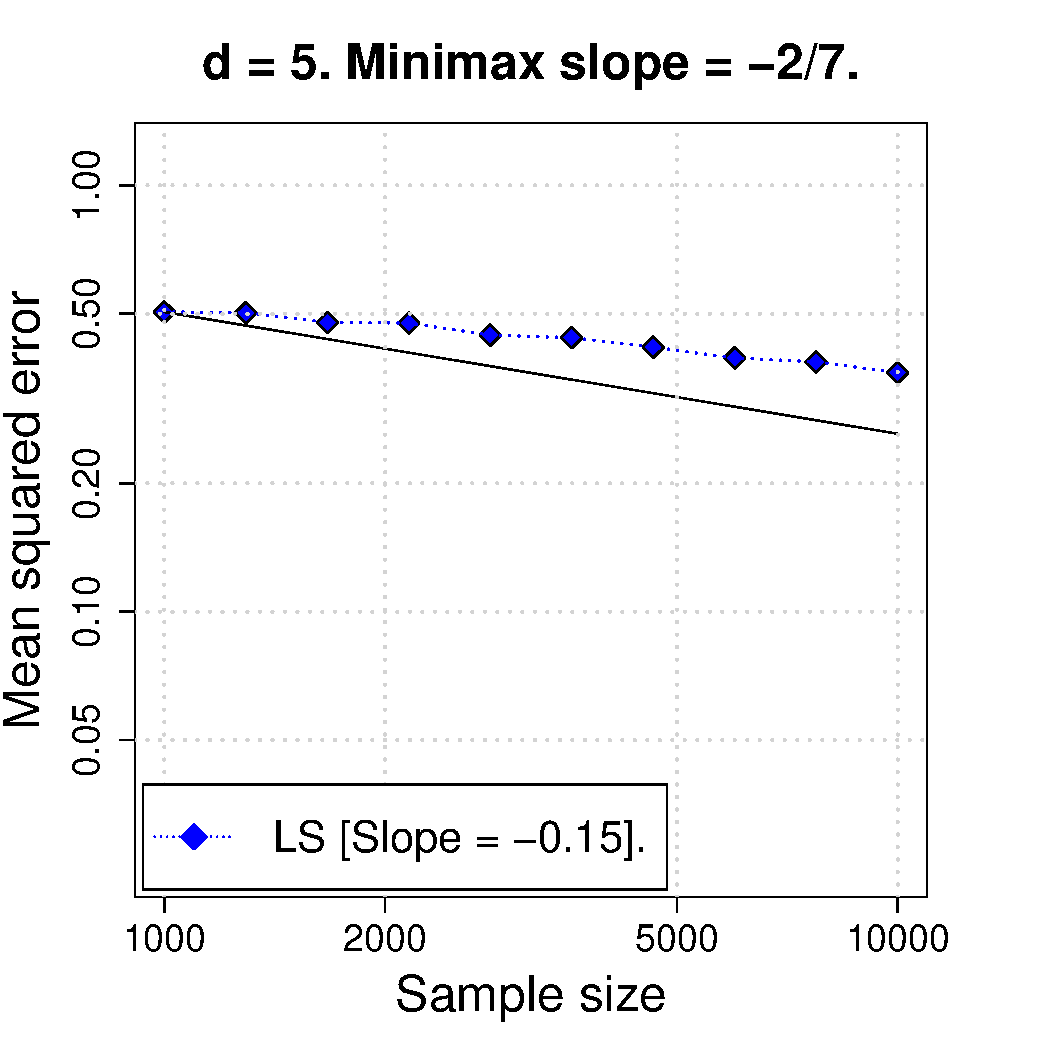
\includegraphics[width=.24\textwidth]{figures/cosine/mse_by_sample_size_5d.pdf}
\end{figure}

\alert{Testing}: Sobolev class $H^1$ does not embed into $L^4$ (Sobolev Embedding Theorem). Usual test statistics may not have a variance.
\end{frame}

\begin{frame}{Extensions}
Several different directions.
\begin{itemize}
	\item \alert{Manifold adaptivity}: When $p$ has support on a manifold of dimension $m < d$, optimal rates are \blue{$n^{-2/(2 + m)}$} (estimation) and \blue{$n^{-4/(4 + m)}$} (testing). Does Laplacian smoothing automatically adapt? \blue{(Yes! See paper.)} 
	\item \alert{Out-of-sample estimation}: Can we extend estimator $\wh{f}$ to have optimal out-of-sample mean squared error? \blue{(Yes, if $f_0$ is Lipschitz! See paper.)}
	\item \alert{Smoothness adaptivity}: When $f_0$ has $s$ smooth derivatives, optimal rates are \blue{$n^{-2s/(2s + m)}$} (estimation) and \blue{$n^{-4s/(4s + m)}$} (testing). Does Laplacian smoothing adapt? (Future work...)
	\item \alert{Different methods}: Spectral cutoff? $k$NN graph? Normalized Laplacian? (Future work...)
\end{itemize}
\end{frame}

\begin{frame}[t]{Summary}
	Specific takeaway: Laplacian smoothing is an optimal method for nonparametric regression. \newline
	
	General takeaway: Discretization can allow us to solve problems even when their continuum analogues are not well-posed.
	\newline 
	\newline
	\newline
	
	\begin{center}
	{\huge Thank You!}
	\end{center}
	
	
\end{frame}

\begin{frame}{Analysis}
\end{frame}



\end{document}
